\documentclass[tikz]{standalone}
\usepackage{tikz}
\begin{document}

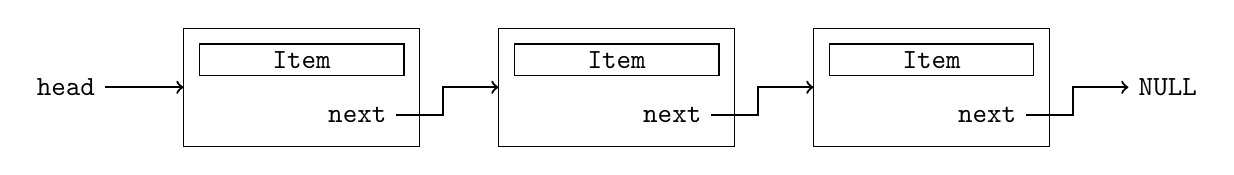
\begin{tikzpicture}[every node/.style={font=\ttfamily}, x=1cm, y=1cm]

% Node 1 (full box)
\draw (0, 0) rectangle (3, 1.5);
% Inner Item box
\draw (0.2, 0.9) rectangle (2.8, 1.3);
\node at (1.5, 1.1) {Item}; % centered Item
% Next label (right-aligned)
\node[anchor=east] (next1) at (2.7, 0.4) {next};

% Node 2 (full box)
\draw (4, 0) rectangle (7, 1.5);
\draw (4.2, 0.9) rectangle (6.8, 1.3);
\node at (5.5, 1.1) {Item};
\node[anchor=east] (next2) at (6.7, 0.4) {next};

% Node 3 (full box)
\draw (8, 0) rectangle (11, 1.5);
\draw (8.2, 0.9) rectangle (10.8, 1.3);
\node at (9.5, 1.1) {Item};
\node[anchor=east] (next3) at (10.7, 0.4) {next};

% NULL
\node at (12.5, 0.75) {NULL};

% head arrow
\draw[->, thick] (-1, 0.75) -- (0, 0.75);
\node[anchor=east] at (-1, 0.75) {head};

% Elbow arrows (from next to next node)
\draw[->, thick] (next1.east) -- ++(+0.6, 0) |- (4, 0.75);
\draw[->, thick] (next2.east) -- ++(+0.6, 0) |- (8, 0.75);
\draw[->, thick] (next3.east) -- ++(+0.6, 0) |- (12, 0.75);

\end{tikzpicture}

\end{document}
